\label{c:Background}
\section{Definitions}
This section covers and differentiates between the basic non-mathematical definitions and terms used in this thesis.

\subsection{Virtual and Augmented Reality}\label{sec:VAR}
The words virtual reality (VR) and augmented reality (AR) can be constantly read in the recent news all over the internet and other media. However, they are used in various contexts and are often defined differently. The definition used in this thesis is therefore only one small aspect of the whole field and should help to differentiate between the two concepts. 
\subsubsection{Virtual reality}
Virtual reality\index{Virtual reality} can be defined as \enquote{an electronic simulation in which images are generated in real time (...) from a stored database and displayed in such a way as to facilitate real-time interaction with the database (...).} \cite[p.148]{Latham.1995}

A virtual reality application uses a combination of software and hardware to let the user experience immersion, interaction and imagination (the three I's of virtual reality) in a virtual world. Whereas the first two I's should be clear and understandable, the last one is often underrated or even left out. Since virtual reality only counts on virtual content and given the fact that computer graphics are still not a perfect representation of our \enquote{reality}, the user's imagination is a very important aspect of an application (\cite[p.3 et seq.]{Burdea.2003}).

Typically, a common computer game can not be classified as a virtual reality application unless it includes the collection and usage of other data than only the keyboard and mouse inputs. For this purpose, a VR application often comes with other interfaces such as a head-mounted display (HMD)\index{Head-mounted display} \footnote{The idea of a HMD started with Morton Heilig's  \index{Morton L. Heilig} U.S. patent in 1960 (see \cite{Heilig.1957}). Recent popular models include the \textit{Oculus Rift} (see \cite{Oculus.2016})\index{Head-mounted display!Oculus Rift} and \textit{Google Cardboard} (see \cite{GoogleDev.2016})\index{Head-mounted display!Google Cardboard}. The HMD tracks, amongst other things, the head position and its movement and displays the stereo image.}. An imaginary example for a perfect virtual reality environment is Star Trek's Holodeck, as mentioned before (\autoref{sec:preface}).

\subsubsection{Augmented reality}
\begin{figure}[htbp]
		\centering
		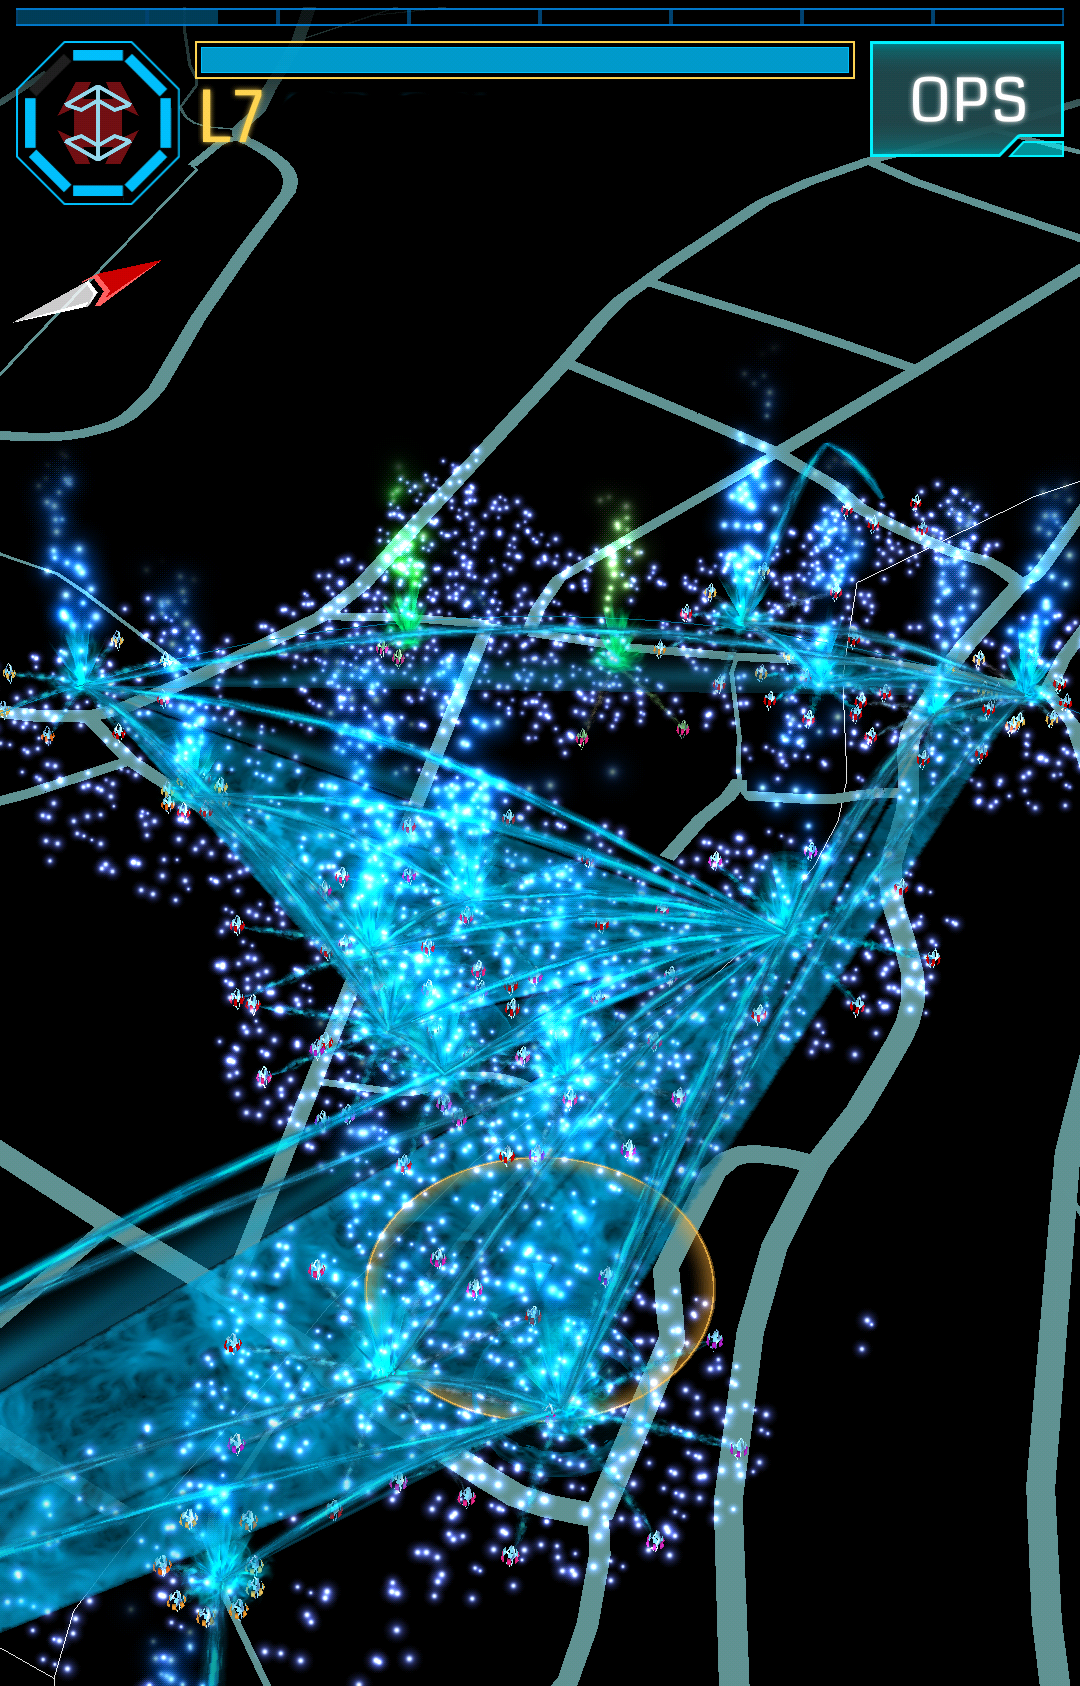
\includegraphics[width=0.4\textwidth]{figures/Ingress}
		\caption[Screenshot of the mobile AR game Ingress]{Screenshot of the mobile AR game Ingress showing the portals around the Hochschule Furtwangen University (\textit{source:} \cite{Haefele.2014}).}
		\label{fig:Ingress}
\end{figure}
In comparison to virtual reality, augmented reality \index{Augmented reality} extends our \enquote{real world} with virtual (digital) content, which must be embedded seamlessly to provide a fully immersive experience. The users can interact with virtual objects and can be provided with relevant additional information about their environment. The virtual data is computed in real-time and is displayed as an overlay on top of the \enquote{real world} in front of the user's eyes. AR highly relies on its technologies. Relevant topics, amongst others, are object recognition, location tracking, interfaces\footnote{A common interface for AR was and still is the head-up display (HUD)\index{Head-up display}, often used for military application (see \cite[p.6]{Burdea.2003}). But also immaterial displays, such as fog screens, are researched (see \cite[p.25 et seq.]{Toennis.2010}).} and real-time computation (compare with \cite[p.1 et seqq.]{Toennis.2010}). 

The game \textit{Ingress}\index{Ingress} by \textit{Niantic, Inc.} (see \autoref{fig:Ingress} for a screenshot), in which two factions fight over virtual portals, is an example for a location-based mobile AR game. The portals, which are linked to real places all over the world, and other game functions are displayed on the user's mobile device in real-time. The users travel to these real places to conquer or defend the portals in the name of their faction (\cite{Niantic.2016}). 

\subsection{Computer vision}\label{ssec:cv}
Computer vision\index{Computer vision} (also referred to as \enquote{machine vision}) is the \enquote{automated extraction of information from images} (\cite{Lowe.2016}). It also refers to a whole field of science, which combines several disciplines\footnote{Among which are mathematics, computer science, as well as phsyics, the psychology of perception and the neuro sciences (\cite[p.xi]{Hartley.2011}).} to research how to make a computer see. Computer vision is differentiated from the wide field of image processing, in which images are processed in different ways to produce new images (compare with \cite{Lowe.2016}).
 
As already stated in the preface, the visual modeling of perception was, for many years, underestimated by scientists studying Artificial Intelligence. Although it is still unclear whether computer vision should be modeled on the basis of biological systems, understanding how biological vision in general, and human depth perception in particular function, seems to be a necessity\footnote{Attempts to find new approaches have not yet been successful.} (compare with \textit{Oliver Faugeras'} foreword in \cite[p.xi]{Hartley.2011}). For this a short overview shall be given in \autoref{ssec:hv}.  

One of the research fields in Computer Vision is the 3-D reconstruction from image data (other fields are listed in \autoref{ssec:Today}). Two important procedures to reconstruct scenes are \textit{structure from motion}\index{Structure from motion} and \textit{stereo correspondence} algorithms. The former uses multiple views of one or more cameras to reconstruct scenes and the latter is described in more detail in the following chapters, since it was used in this thesis.

\subsection{Human Depth Perception}\label{ssec:hv}
Our three-dimensional perception is actually based on a two-dimensional image which is projected onto our retina, but from these 2-D images we are still able to get information about how far away an object is. This information is called \textit{depth cues}\index{Depth cues}, whose connection to the actual depth of field we learn from experience. Depth cues need to be applied to stereoscopic videos to create more accurate depth results (\cite[p.226]{Goldstein.2015} and \cite[p.28]{Hottong.2009}). 

These depth cues can be classified into three different groups (freely adapted from \cite[p.226 et seqq.]{Goldstein.2015} and \cite[p.28 et seqq.]{Hottong.2009}):
\begin{description}
\item [i Oculomotor depth cues\index{Depth cues!Oculomotor depth cues}]\hfill \\ These cues provide depth information for objects which are in closer range (one meter or below). Our brain receives and analyzes feedback from the eye muscles which are contracted differently depending on the distance of the object which gets focused on. We can subconsciously \textit{feel} the muscles' contraction and draw conclusions from it. The oculomotor cues are based on two factors: \textit{accommodation}\index{Depth cues!Accommodation} and \textit{convergence}\index{Depth cues!Convergence}\footnote{The former is based on the contraction of the ciliary muscles, which allow the lens of the eye to take on different shapes in order to change their focal length. The latter uses the information of the eyes' movement as they converge on a moving object to estimate distances.}.
\item [ii Monocular depth cues\index{Depth cues!Monocular depth cues}]\hfill \\ As the name suggests these depth cues can be perceived even with only a single eye (which is one of the reasons that people with only one eye can still perceive depth). They use the previously mentioned accommodation in combination with \textit{pictorial} as well as \textit{movement-produced depth cues} to estimate depth.
	\begin{description}
	\item [Pictorial depth cues]\index{Depth cues!Pictorial depth cues}\hfill \\ Information about depth which can be displayed in a two-dimensional picture. Among them are (\cite[p.227 et seqq.]{Goldstein.2015}):
		\begin{itemize}
		\item \textit{Occlusion}\index{Depth cues!Occlusion}: An overlapped object seems to be further away than the object in front of it. We can not determine the absolute distance of these objects, since these are only relative cues.
		\item \textit{Elevation}: Relative to the horizon we perceive objects which are closer to it as further away than the ones below or higher than it. 		
		\item \textit{Relative and familiar size}: Two objects with the same size change their perceived size according to their position relative to the observer. Objects which are closer appear larger and vice versa. We use our experience to estimate sizes of objects and their distances to us (\autoref{fig:Perugino} shows the difference in sizes of the people which illustrates relative sizes).
		\item \textit{Perspective}\index{Depth cues!Perspective}: Parallel lines converge in the distance and meet in infinity. This concept was often used by artists of the Renaissance to create the optical illusion of depth in their paintings (see \autoref{fig:Perugino} in which the lines converge towards one vanishing point).
		\item \textit{Aerial perspective}: Objects in the far distance appear to be hazy\footnote{In computer games this phenomenon is often called \textit{distance fog}.} and often times have a blue tone with lower contrasts (note that the painter in \autoref{fig:Perugino} used cool colors for distant objects and warmer colors for the foreground).
		\item \textit{Texture gradient}: Textures appear less detailed the further they are from the observer. At the same time elements appear more dense relative to the distant of the viewer.  
		\item \textit{Shading}: Shadows help us to determine positions and they amplify the three-dimensional appearance of objects. 
		\end{itemize}
	\item [Movement-produced depth cues]\index{Depth cues!Movement-produced depth cues}\hfill \\ With the movement of our head or our whole body we receive more cues to determine depth. One of the most important cues is the \textit{motion parallax}\index{Depth cues!Motion parallax}. This depth cue occurs when we see closer objects pass us in a faster speed and more distant objects in a slower pace. It is also often used in 2-D side-scrolling video games (also called \textit{side-scrollers}\index{Side-scroller}) to illustrate depth of field.
Another movement-produced depth cue is the occlusion of objects due to movement (\cite[p.231 et seq.]{Goldstein.2015}).
\end{description}

\begin{figure}[htbp]
		\centering
		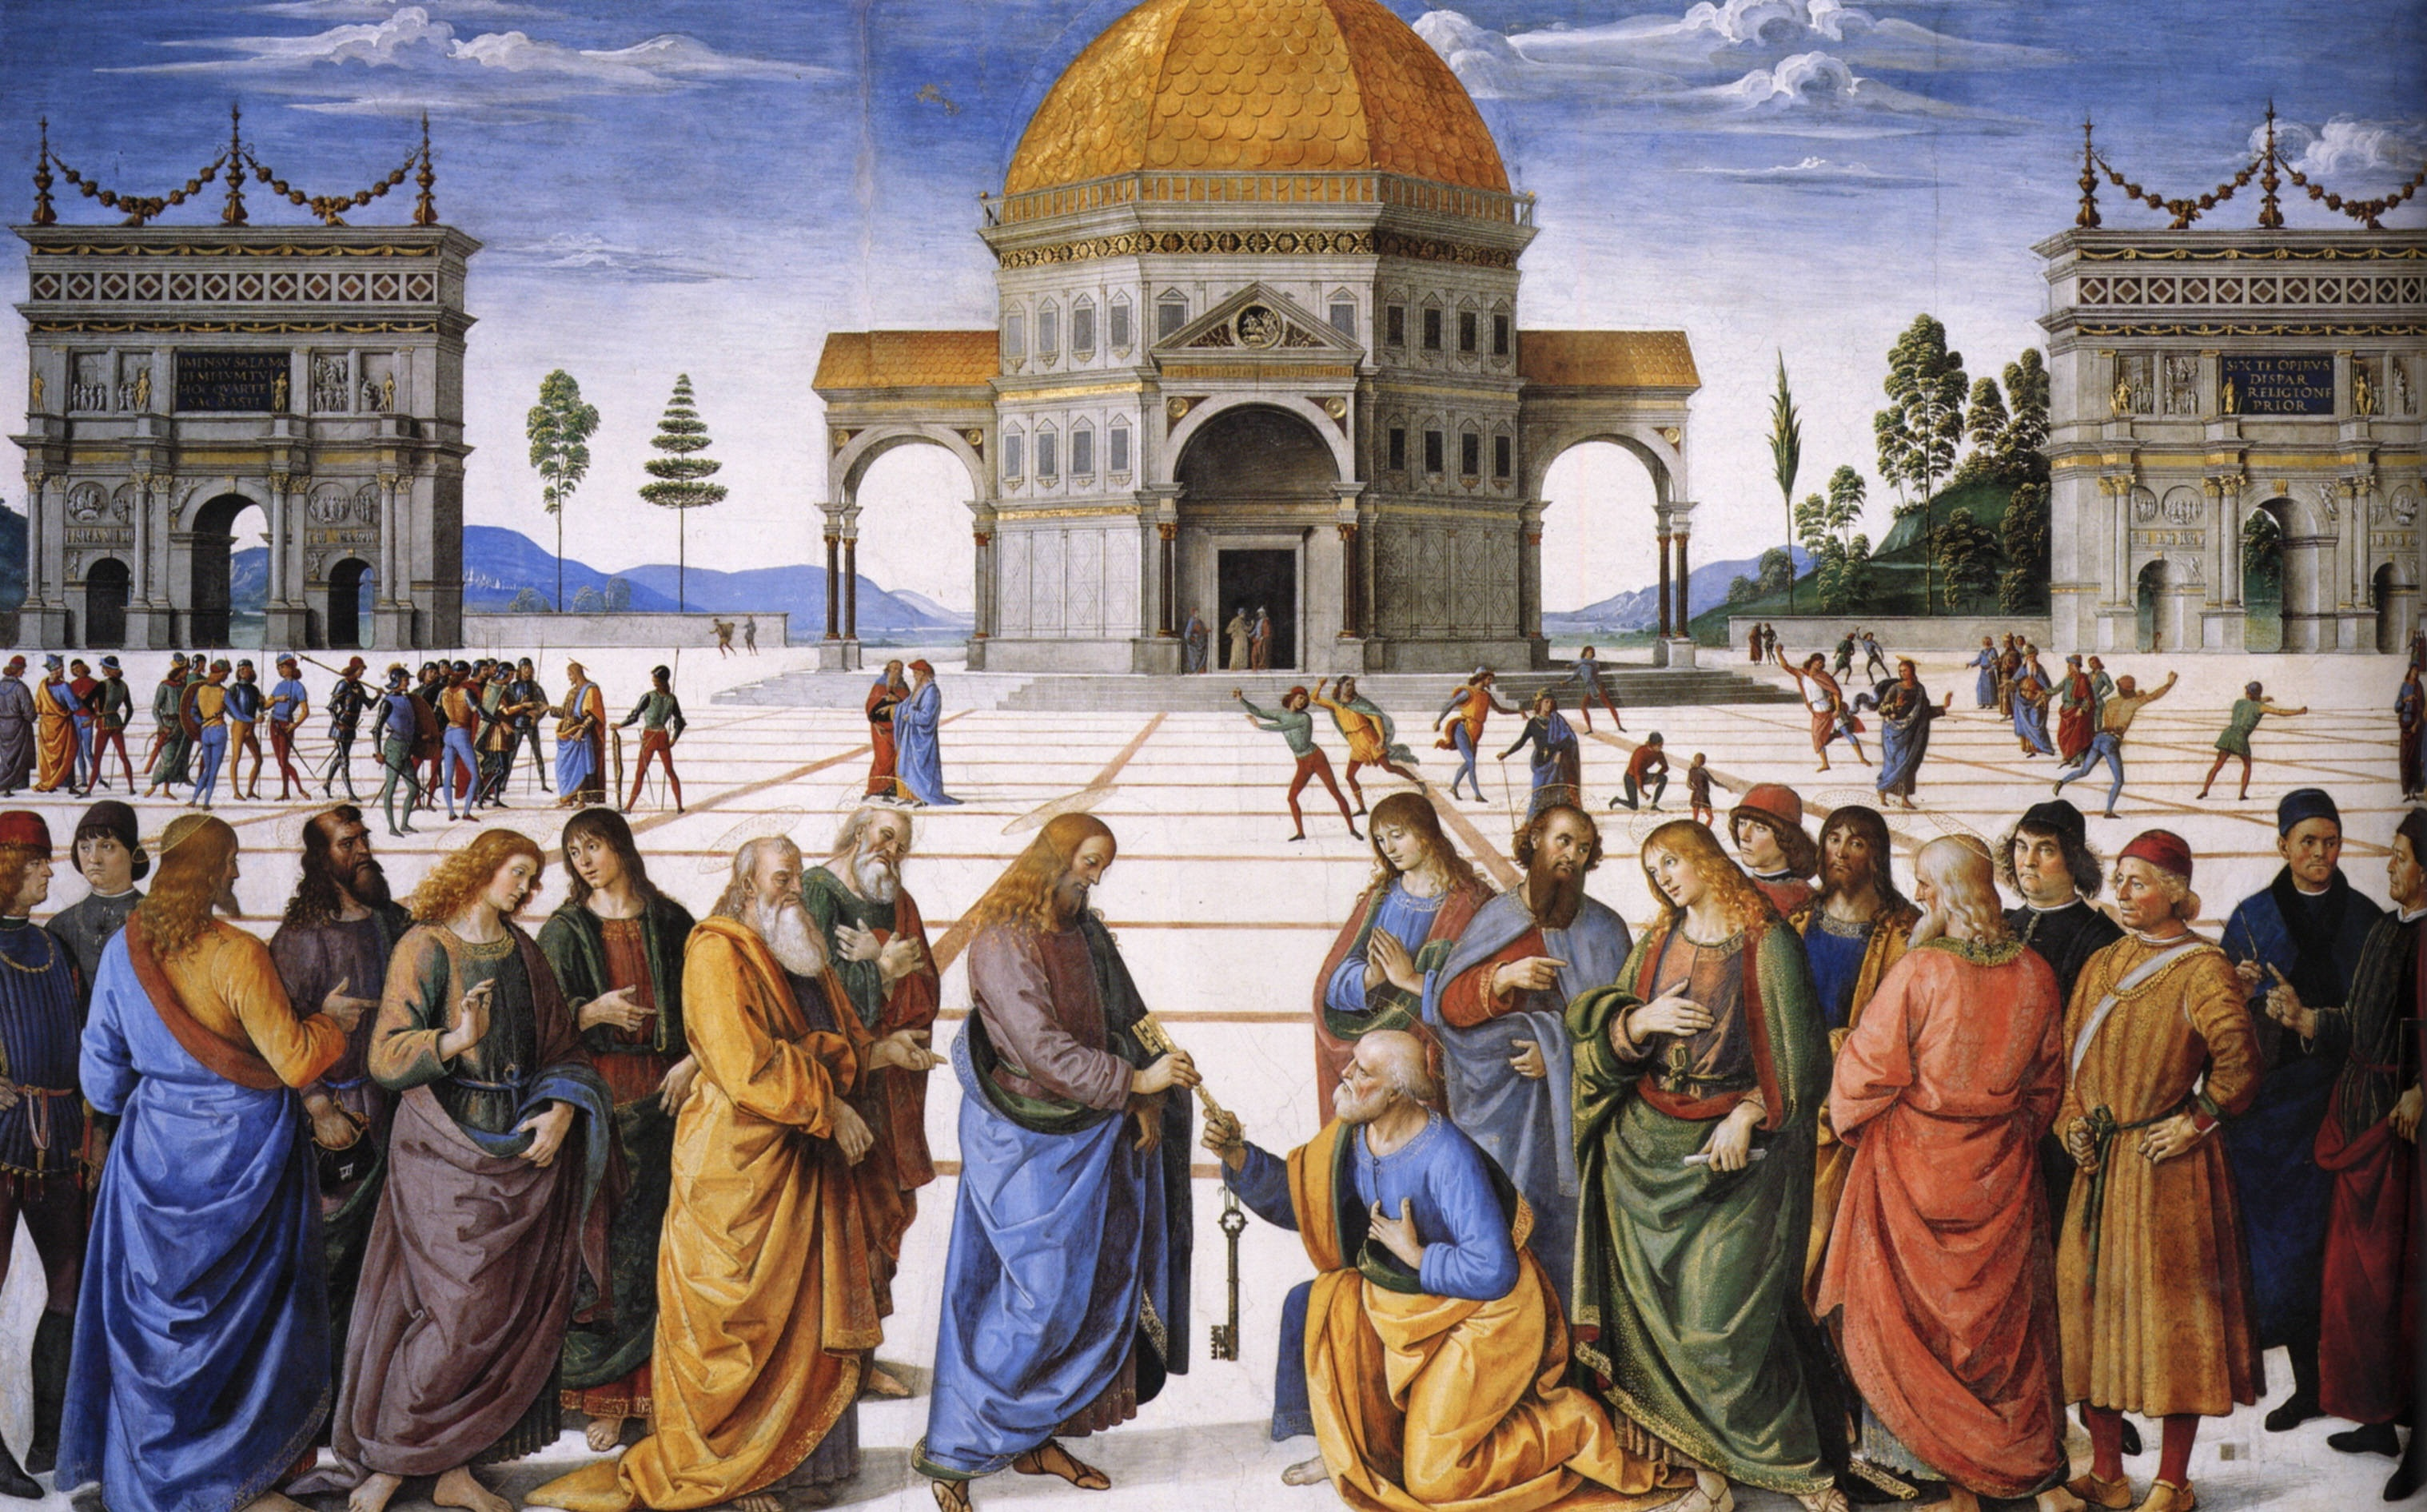
\includegraphics[width=0.8\textwidth]{figures/Perugino-San_Pedro}
		\caption[Pictorial depth cues in Pietro Perugino's fresco \textit{Entrega de las llaves a San Pedro}]{Pictorial depth cues in Pietro Perugino's fresco \textit{Entrega de las llaves a San Pedro} in the Sistine Chapel, Vatican City, 1481-1482}
		\label{fig:Perugino}
\end{figure}

\item [iii Binocular or stereoscopic depth cues\index{Depth cues!Binocular depth cues}]\hfill \\ Stereoscopic depth cues are stimuli for which we need both eyes to experience depth of field. They mainly take the differences between the right and the left image seen by our eyes into account, which makes the interpupillary distance the bases of the stereoscopic vision\footnote{Computer vision algorithms use these principles as a model for creating or analyzing depth with the help of two or more cameras (see \autoref{c:Math} for more details).}.
\end{description}
